%!TeX root = main.tex
\chapter{Elementare meromorphe Zusammenhänge}
\section{Elementare formale meromorphe Zusammenhänge}
\begin{defn}
Ein \emph{elementarer formaler meromorpher Zusammenhang} ist ein Zusammenhang
$\cM$, welcher isomorph zu $\cD_{\hat K}/\cD_{\hat K}\cdot
(x\partial_x-\alpha)^p$, mit passendem $\alpha$ und $p$, ist.
\end{defn}

\begin{lem}
\cite[Lem 5.2.1.]{sabbah_cimpa90}
Es existiert eine Basis von $\cM_{\hat K}$ über $\hat K$ mit der Eigenschaft,
dass die Matrix, die $x\partial_x$ beschreibt, nur Einträge in $\Cfx$ hat.
\end{lem}
\begin{proof}
Wähle einen zyklischen Vektor $m\in\cM_{\hat K}$ % TODO: richtiger Raum?
 und betrachte die Basis $m,\partial_x m,\dots,\partial_x^{d-1}m$ (siehe Lemma
\ref{lem:Zyklischer-Vektor}).
Schreibe $\partial_x^dm=\sum_{i=0}^{d-1}(-b_i(x))\partial_x^im$ in
Basisdarstellung mit Koeffizienten $b_i\in\hat K$.
Also erfüllt $m$ die Gleichung
$\partial_x^dm+\sum_{i=0}^{d-1}b_i(x)\partial_x^im=0$.

\begin{comment} TODO: bis hier schon klar \end{comment}

Tatsächlich kann man $b_i(x)=x^ib_i'(x)$ mit $b_i'\in \Cfx$ schreiben (wegen
Regularität).

Dies impliziert, dass $m,x\partial_xm,\dots,(x\partial_x)^{d-1}m$ ebenfalls
eine Basis von $\cM_{\hat K}$ ist.

Die Matrix von $x\partial_x$ zu dieser neuen Basis hat nur Einträge in $\Cfx$.
\end{proof}
\begin{lem}
\cite[Lem 5.2.2.]{sabbah_cimpa90}
Es existiert sogar eine Basis von $\cM_{\hat K}$ über $\hat K$ so dass die
Matrix zu $x\partial_x$ konstant ist.
\end{lem}
\begin{proof}
Siehe \cite[Thm 5.2.2]{sabbah_cimpa90}
\end{proof}

\begin{thm} \label{thm:regulärInDirSumme}
Ein regulärer formaler Zusammenhang $\cM_{\hat K}$ ist isomorph zu einer
direkten Summe von elementaren formalen meromorphen Zusammenhängen.
\end{thm}
\begin{proof}[Beweisskizze]
Siehe \cite[Cor. 5.2.6]{sabbah_cimpa90}. Man wählt eine Basis von $\cM_{\hat
K}$, in der die Matrix zu $x\partial_x$ konstant ist. Diese Matrix kann
in Jordan Normalform gebracht werden und damit erhält man das Ergebnis.
\end{proof}

\section{Elementare meromorphe Zusammenhänge}
%TODO: rename to L-T-Theorem???
\begin{comment}
einführen als Bausteine oder kleinste meromorphe Zusammenhänge
\end{comment}
\begin{comment}
ALT:
\begin{defn}
\cite[1.a]{sabbah_Fourier-local}
Sei $\phi\in\hat K$.
Wir schreiben $\sE_{\hat K}^\phi$ für den (formalen) Rang 1 Vektorraum $\Cfxl
\bydef \hat K$ ausgestattet mit dem Zusammenhang
$\nabla=\partial_x+\partial_x\phi$, im speziellen also
$\nabla_{\partial_x}1=\partial_x1=\phi'$.\\
\end{defn}
\end{comment}
\begin{defn} \label{defn:rang1Vr}
\cite[1.a]{sabbah_Fourier-local}
Sei $\phi\in\hat K$.
Wir schreiben $\sE_{\hat K}^\phi$ für den (formalen) Rang 1 Vektorraum 
$\bme\cdot\hat K$, wobei $\bme\in\sE_{\hat K}^\phi$ Basis ist, ausgestattet mit
$\partial_x(f\cdot \bme)
=(\frac{\partial f}{\partial x}+f\cdot\frac{\partial\phi}{\partial x})\cdot\bme$, 
im speziellen also $\partial_x\bme=\phi'$.
\end{defn}
\begin{bem}
\begin{enumerate}
\item Die $\sE_{\hat K}^\phi$ stellen so etwas, wie die einfachsten meromorphen
Zusammenhänge mit einem ganzzahligem Slope, dar.
\item Wir werden oft $\bme=1$ als Basis nehmen.
\item Auf die Angabe von des Rang 1 Vektorraums im Subscript wird, falls dieser
klar ist, meist verzichtet.
\item Es ist $\sE^\phi\cong\cD_{\hat K}/\cD_{\hat
K}\cdot(\partial_x-\phi'(x))$, weil für den zyklischen Vektor $1$ gilt, dass
$\partial_x \cdot 1 = \phi'(x) \cdot 1$.
\end{enumerate}
\end{bem}

\begin{lem}
Für $\phi(x)=\sum_{i=-p}^\infty a_ix^i\in\hat K$ mit $a_{-p}\neq0$ gilt, dass
$\cP(\sE_{\hat K}^\phi)=
\begin{cases}
\{p\} &\text{, wenn }p\geq0
\\\{0\} &\text{, wenn }p<0
\end{cases}
$.
\end{lem}
\begin{proof} 
Es ist 
\begin{align*}
\phi'(x) &=\sum_{i=-p}^\infty ia_ix^{i-1}
\\&=\sum_{i=-{p+1}}^\infty (i+1)a_{i+1}x^{i}
\\&=\underset{\neq0}{\underbrace{-pa_{-p}}}x^{-(p+1)}
  +\sum_{i=-{p}}^\infty (i+1)a_{i+1}x^{i}
\end{align*}
und damit wissen wir, dass die einzigen zwei Punkte, die Ecken des Newton
Polygons sein können, $(1,-1)$ und $(0,-(p+1))$ sind. Da einer der Punkte auf
der vertikalen Achse liegt, kann es insgesamt nur einen Slope $\Lambda$ geben,
welcher sich wie folgt berechnet:
\begin{align*}
\Lambda&=\max\{0,\frac{-1-(-(p+1))}{1}\}
\\&=\max\{0,p\}
\\&=\begin{cases}
  p &\text{, wenn }p\geq0
\\0 &\text{, wenn }p<0
\end{cases}
\end{align*}

\iffalse
\begin{figure}[H] % htbp
\begin{center}
  \begin{tikzpicture}[scale=1,descr/.style={fill=white,inner sep=2.5pt}]
  \def\myPoints{0/-6,1/-1}
  \def\myPath{ -- node[descr]{$p$} (1,-1)}
  \myPlotFunction[nogrid]{\myPoints}{\myPath}{1}{-6}{0}{$N(\sE_{\hat K}^\phi)$}
  \end{tikzpicture}
\end{center}
\caption{Newton Polygon zu $\sE_{\hat K}^\phi$}
\end{figure}
\fi
\end{proof}

\begin{comment}
\begin{bem} \label{bem:FormRang1VR}
\cite[1.a]{sabbah_Fourier-local}
Es gilt $\sE^\phi\cong\sE^\psi$ genau dann wenn $\phi\equiv\psi \mod \Cfx$.
\end{bem}
\end{comment}

Sei $\rho:t\mapsto x:=t^p$ und $\mu_\xi:t\mapsto\xi t$.
\begin{lem}
\cite[Lem 2.4]{sabbah_Fourier-local}
Für alle $\phi \in \hat L$ gilt
\[
\rho^+\rho_+\sE^\phi=\bigoplus_{\xi^p=1}\sE^{\phi\circ\mu_\xi} \,.
\]
\end{lem}
%
\begin{proof}
Wir wollen zeigen, dass das folgende Diagramm, für einen passenden
Isomorphismus, kommutiert:
\begin{center}
  \begin{tikzpicture} [scale=3.3, descr/.style={fill=white,inner sep=2.5pt} ]
  \matrix (m) [
    matrix of math nodes
    ,row sep=2em
    ,column sep=6em
    %,text height=3em
    %,text depth=0.25em
    ]
  {
    \rho^+\rho_+\sE^{\phi(u)} &
    \bigoplus_{\xi^p=1}\sE^{\phi\circ\mu_\xi} \\
    \rho^+\rho_+\sE^{\phi(u)} &
    \bigoplus_{\xi^p=1}\sE^{\phi\circ\mu_\xi} \\
  };
    \path[->,font=\scriptsize,>=angle 90]
    (m-1-1) edge node[right]{$\partial_t$} (m-2-1)
    (m-1-2) edge node[right]{$\partial_t$} (m-2-2)
    (m-1-1) edge node[below]{$\cong$} (m-1-2)
    (m-2-1) edge node[below]{$\cong$} (m-2-2)
    ;
  \end{tikzpicture}
\end{center}
Es sei oBdA $\phi\in t^{-1}\C[t^{-1}]$, dies ist nach Bemerkung 
\ref{bem:FormRang1VR} berechtigt.
Wir wählen eine $\hat L$ Basis $\bme$ des Rang 1 $\hat L$-Vektorraum $\sE^\phi$
und damit erhält man die Familie $\bme,t\bme,...,t^{p-1}\bme$ als $\hat
K$-Basis von $\rho_+\sE^\phi$.
Es gilt 
\begin{equation} \label{eq:2-4-basisAbleitung}
\partial_xt^{k}\bme =\rho'(t)^{-1}\underbracket{\partial_tt^{k}}\bme
  =\rho'(t)^{-1}\overbracket{(t^{k}\partial_t + kt^{k-1})}\bme \,.
\end{equation}
Durch die Setzung $\bme_k:=t^{-k}\otimes_{\hat K}t^k\bme$ wird die Familie
$\mathbf{e}:=(\bme_0,...,\bme_{p-1})$ eine $\hat L$-Basis von
$\rho^+\rho_+\sE^\phi$.\\
Zerlege nun 
\begin{align} \label{eq:2-4-gleichung1}
t\phi'(t)&=\sum_{j=0}^{p-1}t^j\psi_j(t^p) &\in t^{-2}\C[t^{-1}]
\end{align}
mit $\psi_j\in\C[x^{-1}]$ für alle $j>0$ und $\psi_0\in x^{-1}\C[x^{-1}]$
(siehe: Anhang \ref{chap:aufteilung}). Damit gilt:
\[
t\partial_t\bme_k= \sum_{i=0}^{p-1-k}t^i\psi_i(t^p)\bme_{k+1} +
  \sum_{i=p-k}^{p-1}t^i\psi_i(t^p)\bme_{k+i-p} 
\]
denn:
\begin{align*}
t\partial_t\bme_k &= 
  t\underbracket{\partial_t(t^{-k}\otimes_{\hat K}t^k\bme)}\\
  &\!\!\overset{(\ref{eq:TensorAbleiten})}{=} 
    t\overbracket{(-kt^{-k-1}\otimes_{\hat K}t^k\bme +
    pt^{p-1}\cdot t^{-k}\otimes_{\hat K}\underbracket{\partial_x
    (\underset{\in\rho_+\sE^\phi}{\underbrace{t^k\bme}})})}\\
  &\!\!\overset{(\ref{eq:2-4-basisAbleitung})}{=} -kt^{-k}\otimes_{\hat K}t^k\bme +
    pt^{p-1}t^{-k+1}\otimes_{\hat K}\overbracket{(pt^{p-1})^{-1} (kt^{k-1}\bme
    + t^k\phi'(t)\bme)}\\
  &= -kt^{-k}\otimes_{\hat K}t^k\bme +
    \underbracket{t^{-k+1}\otimes_{\hat K}(kt^{k-1}\bme + t^k\phi'(t)\bme)}\\
  &= \underset{=0}{\underbrace{-kt^{-k}\otimes_{\hat K}t^k\bme +
    \rlap{$\overbracket{\phantom{x^x\qquad\qquad\qquad\qquad\qquad\qquad\qquad%
      \,\,\,\,\,\,\,\,}}$}
    t^{-k+1}\otimes_{\hat K}kt^{k-1}\bme}} +
    t^{-k+1}\otimes_{\hat K}t^k\phi'(t)\bme\\
  &= t^{-k}\otimes_{\hat K}t^{k}\underbracket{t\phi'(t)}\bme\\
  &\!\!\overset{(\ref{eq:2-4-gleichung1})}{=}t^{-k}\otimes_{\hat K}
    t^{k} \overbracket{\sum_{i=0}^{p-1}t^i\psi_i(t^p)} \bme\\
  &=\sum_{i=0}^{p-1}\psi_i(t^p)(t^{-k}\otimes_{\hat K} t^{k} t^i \bme)\\
  &=\sum_{i=0}^{p-1}t^i\psi_i(t^p)(t^{-k-i}\otimes_{\hat K} t^{k+i} \bme)\\
  &= \sum_{i=0}^{p-1-k}t^i\psi_i(t^p)\bme_{k+i} +
  \sum_{i=p-k}^{p-1}t^i\psi_i(t^p)\bme_{k+i-p} \,.
\end{align*}
Sei
\[
V:=\begin{pmatrix}
0 &        &          & 1\\
1 & 0\\
  & \ddots & \ddots\\
  &        & 1        & 0
\end{pmatrix} \,,
\]
so dass $\mathbf{e}\cdot V=(\bme_1,...,\bme_{p-1},\bme_0)$ gilt.
Es gilt:
\[
t\partial_t\mathbf{e}=\mathbf{e}\left[\sum_{j=0}^{p-1}t^j\psi_jV^j}\right]
\]
denn:
\begin{align*}
  t\partial_t\mathbf{e} &= (t\partial_t\bme_0,...,t\partial_t\bme_{p-1})\\
  &= \Bigg(\sum_{i=0}^{p-1-k}t^i\psi_i(t^p)\bme_{k+1} +
    \sum_{i=p-k}^{p-1}t^i\psi_i(t^p)\bme_{k+i-p}\Bigg)_{k\in\{0,..,p-1\}}\\
  &= \mathbf{e}
{ %\small
  \footnotesize
  \begin{pmatrix}u^{p-1}\psi_{p-1}(t^p) && \cdots & t^{3}\psi_{3}(t^p) & t^{2}
  \psi_{2}(t^p) & t^{1}\psi_{1}(t^p)\\
  t^{1}\psi_{1}(t^p) & t^{p-1}\psi_{p-1}(t^p) &  &
  & \ddots & t^{2}\psi_{2}(t^p)\\
  t^{2}\psi_{2}(t^p) & t^{1}\psi_{1}(t^p) & \ddots &  &  & t^{3}\psi_{3}(t^p)\\
  t^{3}\psi_{3}(t^p) & \ddots & \ddots & \ddots &  & \vdots\\
  \vdots &  & \ddots & t^{1}\psi_{1}(t^p) & t^{p-1}\psi_{p-1}(t^p)\\
  t^{p-2}\psi_{p-2}(t^p) & \cdots & t^{3}\psi_{3}(t^p) & t^{2}\psi_{2}(t^p) &
  t^{1}\psi_{1}(t^p) & t^{p-1}\psi_{p-1}(t^p)
  \end{pmatrix}
} \\
  &= \mathbf{e}\left[\sum_{j=0}^{p-1}t^j\psi_j(t^p)V^j\right] \,.
\end{align*}
Die Wirkung von $\partial_t$ auf die Basis $\mathbf{e}$ von
$\rho^+\rho_+\sE^{\phi(t)}$ ist also beschrieben durch
\[
\partial_t\mathbf{e}=\mathbf{e}\left[\sum_{j=0}^{p-1}t^{j-1}\psi_jV^j\right]\,.
\]
Da $V$ das Minimalpolynom $\chi_V(X)=X^p-1$ hat, können wir diese Matrix durch
Ähnlichkeitstransformation mit $T$ auf die Form
\[
D:=TVT^{-1}=\begin{pmatrix}\xi^{0}\\
 & \xi^{1}\\
 &  & \ddots\\
 &  &  & \xi^{p-1}
\end{pmatrix} \,,
\]
mit $\xi^p=1$, bringen. Sei so ein $\xi$ ab jetzt fixiert. %TODO: besonderes xi?
So dass gilt:
\begin{align*}
  T\left[\sum_{j=0}^{p-1}t^{j-1}\psi_j(t^p)V^j\right]T^{-1} 
  &= \left[\sum_{j=0}^{p-1}t^{j-1}\psi_j(t^p) (TVT^{-1})^j\right]\\
  &= \left[\sum_{j=0}^{p-1}t^{j-1}\psi_j(t^p)D^j\right]\\
  &=
{
  \footnotesize
  \begin{pmatrix}\sum_{j=0}^{p-1}t^{j-1}\psi_{j}(t^p)\\
    & \sum_{j=0}^{p-1}t^{j-1}\psi_{j}(t^p)\left(\xi^{1}\right)^{j}\\
    & & \ddots\\
    &  &  & \sum_{j=0}^{p-1}t^{j-1}\psi_{j}(t^p)\left(\xi^{p-1}\right)^{j}
  \end{pmatrix}
}\\
  &=
{
  \footnotesize
  \begin{pmatrix}\sum_{j=0}^{p-1}t^{j-1}\psi_{j}(t^p)\\
    & \sum_{j=0}^{p-1}(t\xi^1)^{j-1}\psi_{j}(t^p)\xi^{1}\\
    & & \ddots\\
    &  &  & \sum_{j=0}^{p-1}(t\xi^{p-1})^{j-1}\psi_{j}(t^p)\xi^{p-1}
  \end{pmatrix}
}\\
  &= \begin{pmatrix}\phi'(t)\\
    & \phi'(\xi t)\xi^{1}\\
    & & \ddots\\
    &  &  & \phi'(\xi^{p-1} t)\xi^{p-1}
  \end{pmatrix}\\
  &= \begin{pmatrix} pt^{p-1}\\
    & p(\xi t)^{p-1}\xi\\
    & & \ddots\\
    &  &  & p(\xi^{p-1} t)^{p-1}\xi^{p-1}
  \end{pmatrix}\\
\end{align*}
da $\phi'(t)=pt^{p-1}$.
Damit wissen wir bereits, dass im Diagramm
\begin{center}
  \begin{tikzpicture} [scale=3.3, descr/.style={fill=white,inner sep=2.5pt} ]
  \matrix (m) [
    matrix of math nodes
    ,row sep=2em
    ,column sep=9em
    %,text height=3em
    %,text depth=0.25em
    ]
  {
    \rho^+\rho_+\sE^{\phi(u)} &
    \hat L^p &
    \hat L^p &
    \bigoplus_{i=0}^{p-1}\sE^{\phi\circ\mu_{\xi^i}} \\
    & \\
    & \\
    \rho^+\rho_+\sE^{\phi(u)} &
    \hat L^p &
    \hat L^p &
    \bigoplus_{i=0}^{p-1}\sE^{\phi\circ\mu_{\xi^i}} \\
  };
    \path[->,font=\scriptsize,>=angle 90]
    (m-1-2) edge node[below]{$\cong$} (m-1-1)
    (m-1-1) edge node[right]{$\partial_t$} (m-4-1)
    (m-4-2) edge node[below]{$\cong$} (m-4-1)
    (m-1-3) edge node[above]{$T$} node[below]{$\cong$} (m-1-2)
    (m-4-3) edge node[above]{$T$} node[below]{$\cong$} (m-4-2)
    (m-1-2) edge node[descr]{\fbox{$\sum_{j=0}^{p-1}t^{j-1}\psi_j(t^p)V^j$}} 
      (m-4-2)
    (m-1-3) edge node[descr]{\fbox{$\sum_{j=0}^{p-1}t^{j-1}\psi_j(t^p)D^j$}} 
      (m-4-3)
    (m-1-3) edge node[above]{$\Phi$} node[below]{$\cong$} (m-1-4)
    (m-4-3) edge node[above]{$\Phi$} node[below]{$\cong$} (m-4-4)
    (m-1-4) edge node[right]{$\partial_t$} (m-4-4)
    ;

    \draw [decoration={brace,amplitude=10pt},decorate]
      (m.south -| m-4-3.east) -- node[midway,yshift=-0.6cm]{$(\star)$} 
        (m.south -| m-4-1.west);
  \end{tikzpicture}
\end{center}
der mit $(\star)$ bezeichnete Teil kommutiert,
wobei $\Phi:(0,\dots,0,\overbox{1}{k-te Stelle},0,\dots,0)\mapsto e_k$ der
kanonische Basisisomorphismus und $e_k$ Basis von
$\sE^{\phi\circ\mu_{\xi^{k-1}}}$.
Um zu zeigen, dass das vollständige Diagramm kommutiert, zeigen wir noch, dass
\begin{align*}
\partial_t(v) =\Phi\big(\Phi^{-1}(v)
  \cdot\left[\sum_{j=0}^{p-1}t^{j-1}\psi_j(t^p)D^j\right]\big)
& & \forall v\in \bigoplus_{i=0}^{p-1}\sE^{\phi\circ\mu_{\xi^i}} \\
\end{align*}
gilt. Es reicht zu zeigen, dass die Aussage für alle Basiselemente $e_k$ gilt.
Nach Definition \ref{defn:rang1Vr} gilt
\begin{align*}
\partial_t e_k &= \underbracket{(\phi\circ\mu_{\xi^{k-1}})'(t)}e_k
\\&\overbox{=}{Kettenregel}
  \overbracket{\underbracket{\phi(\mu_{\xi^{k-1}}')}
  \cdot\underbracket{\phi'(t)}}e_k
\\&=\overbracket{(\xi^{k-1})^p}\cdot\overbracket{(pt^{p-1})}e_k
\\&=p(\xi^{k-1}t)^{p-1}\xi^{k-1}e_k
\end{align*}
und auf dem anderem Weg gilt:
\begin{center}
  \begin{tikzpicture} [scale=3.3, descr/.style={fill=white,inner sep=2.5pt} ]
  \matrix (m) [
    matrix of math nodes
    ,row sep=7em
    ,column sep=9em
    ]
  {
    \Phi^{-1}(e_k)=(\dots,0,1,0,\dots) & e_k\\
    (\dots,0,p (\xi^{k-1} t)^{p-1},0,\dots) &
    \phi'(\xi^{k-1} t)\xi^{k-1} e_k \\
  };
    \path[|->,font=\scriptsize,>=angle 90]
    (m-1-2) edge node[above]{$\Phi^{-1}$} (m-1-1)
    (m-1-1) edge node[descr]{\fbox{$\sum_{j=0}^{p-1}t^{j-1}\psi_j(t^p)D^j$}} 
      (m-2-1)
    (m-2-1) edge node[above]{$\Phi$} (m-2-2)
    ;
  \end{tikzpicture}
\end{center}
Also kommutiert das Diagramm und damit ist die Aussage gezeigt.
\end{proof}

\begin{defn}
Ein \emph{elementarer meromorpher Zusammenhang} ist ein Zusammenhang $\cM$, für
den es $\psi \in \Cfxl$, $\alpha\in\C$ und $p\in \N$ gibt, so dass
\[
\cM\cong \sE^{\psi}\otimes R_{\alpha,p}\,,
\]
mit $R_{\alpha,p}:=\cD/\cD(x\partial_x-\alpha)^p$, also ein elementarer
formaler meromorpher Zusammenhang, ist.
\end{defn}

\begin{comment}
\begin{lem}
$\sE^{\psi}\otimes R_{\alpha,p}\cong
\cD/\cD\cdot(x\partial_x-(\alpha+x\frac{\partial \psi}{\partial x}))^p$
\end{lem}
\begin{proof}
Siehe \cite[Lem 5.12]{DiplHedwig}
\end{proof}
\end{comment}

\begin{comment}
\section{Definition in \cite{sabbah_Fourier-local}}
%TODO: auch nicht formal
\begin{defn}[Elementarer formaler Zusammenhang]
\cite[Def 2.1]{sabbah_Fourier-local}
Zu einem gegebenen $\rho\in t\C\llbracket t\rrbracket$, $\phi\in \hat L \bydef
\C(\!(t)\!)$ und einem endlich dimensionalen $\hat L$-Vektorraum $R$ mit
regulärem Zusammenhang $\nabla$, definieren wir den assoziierten elementaren
endlich dimensionalen $\hat K$-Vektorraum mit Zusammenhang, durch:
\[
El(\rho,\phi,R)=\rho_+(\sE^\phi\otimes R)
\]
\end{defn}
\cite[nach Def 2.1]{sabbah_Fourier-local}
Bis auf Isomorphismus hängt $El(\rho,\phi,R)$ nur von $\phi\mod\Cft$ ab.
\begin{lem}
\cite[Lem 2.2]{sabbah_Fourier-local}
\end{lem}
\begin{lem} \cite[Lem 2.6.]{sabbah_Fourier-local}
Es gilt $El([t\mapsto t^p],\phi,R)\cong El([t\mapsto t^p],\psi,S)$ genau dann,
wenn
\begin{itemize}
\item es ein $\zeta$ gibt, mit $\zeta^p=1$ und
$\psi\circ\mu_\zeta\equiv\phi\mod\Cft$
\item und $S\cong R$ als $\hat L$-Vektorräume mit Zusammenhang.
\end{itemize}
\end{lem}
\begin{proof}
Siehe \cite[Lem 2.6.]{sabbah_Fourier-local}
\end{proof}
%
\begin{prop} \cite[Prop 3.1]{sabbah_Fourier-local}
Jeder irreduzible endlich dimensionale $\hat K$-Vektorraum $\cM$ mit
Zusammenhang ist isomorph zu $\rho_+(\sE^\phi\otimes L)$, wobei $\phi\in
t^{-1}\C[t^{-1}]$, $\rho:t\rightarrow t^p$ vom Grad $p\geq 1$ und ist minimal
unter $\phi$. (siehe \cite[Rem  2.8]{sabbah_Fourier-local}) und $L$ ist ein
Rang $1$ $\hat L$-Vektrorraum mit regulärem Zusammenhang.
\end{prop}
\begin{proof}
%TODO: verwendet hier schon das klassische Levelt-Turittin
Siehe \cite[Prop 3.1]{sabbah_Fourier-local}
\end{proof}
\end{comment}

\section{Twisten von meromorphen Zusammenhängen}
\begin{comment}
\cite[Chap 5 §2]{coutinho1995primer}
\end{comment}
\begin{lem}
Sei $\cM=\cD_{\hat K}/\cD_{\hat K}\cdot P$ ein meromorpher Zusammenhang mit $P$
von Grad $q$ und mit $\bme$ als ein zyklischer Vektor, so ist $\bme\otimes
\underset{\in\hat K}{\underbrace{1}}$ ein zyklischer Vektor für
$\cN:=\cM\otimes_{\hat K}\sE_{\hat K}^\psi$.
\end{lem}
\begin{proof}
%Es sei $\bme$ ein zyklischer Vektor von $\cM$.
Da der Grad von $P$ gleich $q$ ist, ist nach Lemma \ref{lem:twistRechenregel}
auch $Q$ von grad $q$ und somit $\dim_{\hat K}\cN= q$.
Also reicht es zu zeigen, dass $\bme\otimes 1$, $\partial_x(\bme\otimes 1)$,
$\partial_x^2(\bme\otimes 1)$,\dots, $\partial_x^{q-1}(\bme\otimes 1)$ ein
linear unabhängiges System ist.  Es gilt
\begin{align*}
\partial_x(\bme\otimes 1) &= (\partial_x \bme)\otimes 1 + x\otimes \partial_x 1\\
  &= (\partial_x \bme)\otimes 1 + \bme\otimes \psi'(x)\\
  &= (\partial_x \bme)\otimes 1 +  \psi'(x)(\bme\otimes 1)\\
\partial_x^2(\bme\otimes 1) &= \partial_x((\partial_x \bme)\otimes 1 +
    \psi'(x)(\bme\otimes 1))\\
  &= (\partial_x^2 \bme)\otimes 1 + (\partial_x \bme)\otimes \psi'(x)
  + \psi''(x)(\bme\otimes 1)
  + \psi'(x)((\partial_x \bme)\otimes 1 + \bme\otimes \psi'(x))\\
  &= (\partial_x^2 \bme)\otimes 1
  + \psi'(x)(\partial_x \bme)\otimes 1
  + \psi''(x)(\bme\otimes 1)
  + \psi'(x)(\partial_x \bme)\otimes 1
  + \psi'(x)^2(\bme\otimes 1)\\
  &= (\partial_x^2 \bme)\otimes 1
  + 2\psi'(x)(\partial_x \bme)\otimes 1
  + (\psi''(x) + \psi'(x)^2)(\bme\otimes 1)\\
  &\,\,\,\vdots\\
\partial_x^{q-1}(\bme\otimes 1) &= (\partial_x^{q-1} \bme)\otimes 1
  + \lambda_{q-2}(\partial_x^{q-2} \bme)\otimes 1
  +\dots
  + \lambda_{1}(\partial_x \bme)\otimes 1
  + \lambda_0(\bme\otimes 1)\\
\end{align*}
und somit ist dann
\[
\begin{pmatrix}
\bme\otimes 1\\
\partial_x(\bme\otimes 1)\\
\partial_x^2(\bme\otimes 1)\\
\vdots\\
\partial_x^{q-2}(\bme\otimes 1)\\
\partial_x^{q-1}(\bme\otimes 1)\\
\end{pmatrix}
=
\begin{pmatrix}
1         & 0         & \cdots & \cdots & \cdots        & 0 \\
\psi'(x)  & 1         & 0      &        &               & \vdots\\
\star     & \star     & 1      & 0      &               & \vdots\\
\vdots    &           & \ddots & \ddots & \ddots        & \vdots\\
\star     & \cdots    & \cdots & \star  & 1             & 0\\
\lambda_0 & \lambda_1 & \cdots & \cdots & \lambda_{q-2} & 1\\
\end{pmatrix}
\begin{pmatrix}
\bme\otimes 1\\
(\partial_x \bme)\otimes 1\\
(\partial_x^{2}\bme)\otimes 1\\
\vdots\\
(\partial_x^{q-2}\bme)\otimes 1\\
(\partial_x^{q-1}\bme)\otimes 1\\
\end{pmatrix}
\,.
\]
Da bekanntlich $\bme\otimes1$, $(\partial_x \bme)\otimes 1$,
$(\partial_x^{2}\bme)\otimes 1$,\dots, $(\partial_x^{q-1}\bme)\otimes 1$ linear
unabhängig sind, gilt dies auch für $\bme\otimes 1$, $\partial_x(\bme\otimes
1)$, $\partial_x^2(\bme\otimes 1)$,\dots, $\partial_x^{q-1}(\bme\otimes 1)$.
Damit folgt die Behauptung.
\end{proof}
\begin{lem} \label{lem:twistRechenregel}
Sei $\cM_{\hat K}=\cD_{\hat K}/\cD_{\hat K}\cdot P(x,\partial_x)$ und sei
$\phi\in \hat K$. So gilt
\[
\cM_{\hat K}\otimes_{\hat K}\sE^{\phi}=\cD_{\hat K}/\cD_{\hat K}\cdot
Q(x,\partial_x)
\]
mit $Q(x,\partial_x)=P(x,\partial_x-\frac{\partial \phi}{\partial x})$.
\end{lem}
\begin{proof}[Beweisskizze]
Zeige, dass $P(x,\partial_x-\frac{\partial \phi}{\partial x})\bme\otimes1=0$
gilt, da $\bme\otimes1$ eine zyklischer Vektor folgt damit aus Gradgründen die
Behauptung. Genauer ausgeführt wird dies in 
\cite[Seiten 39 bis 44]{DiplHedwig}.
\begin{comment}
\begin{align*}
P(x,\partial_x-\frac{\partial \phi}{\partial x})\bme\otimes1
 &=TODO
\end{align*}
\end{comment}
\end{proof}
\begin{cor} \label{cor:zurücktwisten}
Sei $\cM_{\hat K}$ und $\phi$ wie in \ref{lem:twistRechenregel}, so gilt
\[
\cM_{\hat K}\otimes_{\hat K}\sE^{\phi}\otimes_{\hat K}\sE^{-\phi}=\cM_{\hat K}\,.
\]
\end{cor}
\begin{proof}
Denn
\begin{align*}
\cM_{\hat K}\otimes_{\hat K}\sE^{\phi}\otimes_{\hat K}\sE^{-\phi}
  &= \cD_{\hat K}/\cD_{\hat K}\cdot P(x,\partial_x)
    \otimes_{\hat K}\sE^{\phi}\otimes_{\hat K}\sE^{-\phi}
\\&= \cD_{\hat K}/\cD_{\hat K}
  \cdot P(x,\partial_x-\frac{\partial \phi}{\partial x})
  \otimes_{\hat K}\sE^{-\phi}
\\&= \cD_{\hat K}/\cD_{\hat K} \cdot P(x,\partial_x\underset{=0}{\underbrace{
  -\frac{\partial \phi}{\partial x} -\frac{\partial (-\phi)}{\partial x}}})
\\&= \cD_{\hat K}/\cD_{\hat K} \cdot P(x,\partial_x) = \cM_{\hat K} \,.
\end{align*}
\end{proof}

\section{Levelt-\!Turrittin-\!Theorem}
Das Levelt-Turrittin-Theorem ist ein Satz, der hilft, meromorphe Zusammenhänge
in ihre irreduziblen Komponenten zu zerlegen.

\begin{comment}
\subsection{Klassische Version}
\end{comment}
\begin{thm}
\cite[Thm 5.4.7]{sabbah_cimpa90}
Sei $\cM_{\hat K}$ ein formaler meromorpher Zusammenhang, so gibt es eine
ganze Zahl $p$, so dass der Zusammenhang $\cM_{\hat L}:=\rho^+\cM_{\hat K}$,
mit $\rho:t\mapsto x:=t^p$, isomorph zu einer direkten Summe von formalen
elementaren meromorphen Zusammenhänge
ist.
\end{thm}
Der folgende Beweis stammt hauptsächlich aus \cite[Seite 35]{sabbah_cimpa90}.
\begin{proof}
Zum Beweis wird Induktion auf die lexicographisch geordnetem Paare
$(\dim_{\hat K}\cM_{\hat K},\kappa)$ angewendet. Wobei
$\kappa\in\N\cup\{\infty\}$ dem größtem Slope von $\cM_{\hat K}$ entspricht. Es
wird $\kappa=\infty$ gesetzt, falls der größte Slope nicht ganzzahlig ist.

\begin{comment}
TODO: Induktionsanfang und -schritt kennzeichnen
\end{comment}
Wir nehmen oBdA an, dass $\cM_{\hat K}$ genau einen Slope $\Lambda$ hat, sonst
Teile $\cM_{\hat K}$ mittels Satz \ref{thm:Split-after-slopes} in meromorphe
Zusammenhänge mit je einem Slope und wende jeweils die Induktion an.
Mit $\Lambda=:\frac{\lambda_0}{\lambda_1}$ (vollständig gekürtzt) definieren
wir die dem Slope entsprechende Linearform
$L(s_0,s_1):=\lambda_0s_0+\lambda_1s_1$.  Wir nennen $\sigma_L(P)\in \hat
K[\xi]$ die \emph{Determinanten Gleichung} von $P$. Da $L$ zu einem Slope von
$P$ gehört, besteht $\sigma_L(P)$ aus zumindest zwei Monomen.
\begin{comment}
and is homogeneous of degree $\ord_L(P)=0$ because $P$ is chosen with
coefficients in $\Cfx$, one of them, being a unit.
\end{comment}
Schreibe
\begin{align*}
\sigma_L(P)&=\sum_{L(i,i-j)=\ord_L(P)}\alpha_{ij}x^j\xi^i\\
  &=\sum_{L(i,i-j)=0}\alpha_{ij}x^j\xi^i \,.
\end{align*}
Sei $\theta:=x^{\lambda_0+\lambda_1}}xi^{\lambda_1}$ so können wir
\[
\sigma_L(P) = \sum_{k\geq 0}\alpha_k\theta^k
\]
schreiben, wobei $\alpha_0\neq0$ ist.

\paragraph{Erster Fall: $\lambda_1=1$.} Das bedeutet, dass der Slope ganzzahlig
ist. Betrachte die Faktorisierung
\[
\sigma_L(P)=\epsilon\prod_{\beta}(\theta-\beta)^{\gamma_\beta}\,.
\]
Wobei $\epsilon\in\C$ eine Konstante ist.  Sei $\beta_0$  eine der Nullstellen,
so setze $R(z):=(\beta_0/(\lambda_0+1))z^{\lambda_0+1}$ und betrachte
$\cM_{\hat K}\otimes \cF_{\hat K}^R$.
\begin{comment}
AB HIER VLT NICHT RICHTIG, nur versuch
\end{comment}
Falls $P(x,\partial_x)\cdot e=0$ gilt
\[
P\Big(x,\partial_x-\frac{\partial R(x^{-1})}{\partial x}\Big)
  \cdot e\otimes e(R)=0
\]
und hier haben wir 
\begin{align*}
\frac{\partial R(x^{-1})}{\partial x} 
  &=\frac{\partial(\frac{\beta_0}{\lambda_0+1}x^{-(\lambda_0+1)})}{\partial
  x}\\
  &=-\beta_0z^{-(\lambda_0+2)} \,.
\end{align*}
Schreibe $P'=P(x,\partial_x+\beta_0x^{-(\lambda_0+2)})$.
\begin{lem}
Es gilt, dass $P'$ Koeffizienten in $\Cfx$ hat.
\end{lem}
\begin{proof}
TODO
\end{proof}
Des weiteren ist $\sigma_L(P')=\sum_{k\geq 0}\alpha_k(\theta+\beta_0)^k$. Wir
unterscheiden nun 2 Unterfälle:
\begin{enumerate}
\item \textbf{Die Determinanten Gleichung $\sigma_L(P)$ hat nur eine
Nullstelle.}
\begin{comment}TODO: Hier weiter \end{comment}
\item \textbf{Die Determinanten Gleichung $\sigma_L(P)$ hat mehrere
Nullstellen.}
\begin{comment}TODO: Hier weiter \end{comment}
\end{enumerate}

\paragraph{Zweiter Fall: $\lambda_1\neq1$.} In diesem Fall ist einzige Slope
$\Lambda$ nicht ganzzahlig. Mache deshalb einen pull-back mit $\lambda_1$. Sei
$\rho:t\mapsto x:=t^{\lambda_1}$ und erhalte $P'$ so dass $\rho^*\cM_{\hat
K}=\cD_{\hat L}/\cD_{\hat L}\cdot P'$.
Nach Lemma \ref{lem:slope-pb-multiplikation} hat $P'$ den einen Slope
$\Lambda\cdot\lambda_1=\lambda_0$.
Damit können wir nun die zugehörige Linearform $L':=\lambda_0s_0+s_1$
definieren. Es gilt dass
\[
\sigma_{L'}(P')=\dots
\]
ist, welches zumindest zwei unterschiedliche Nullstellen hat. Nun wendet man
den zweiten Unterfall des ersten Fall an.

\end{proof} % ende von beweis zu levelt aus sabbah_cimpa90

\begin{comment}
\subsection{Sabbah's Refined version}
\begin{prop}
\cite[Prop 3.1]{sabbah_Fourier-local}
Jeder irreduzible endlich dimensionale formale meromorphe Zusammenhang
$\cM_{\hat L}$ ist isomorph zu $\rho_+(\sE^\phi\otimes_{\hat K} S)$, wobei
$\phi\in x^{-1}\C[x^-1]$, $\rho:x\mapsto t=x^p$ mit grad $p\geq1$ minimal bzgl.
$\phi$ (siehe \cite[Rem 2.8]{sabbah_Fourier-local}), und $S$ ist ein Rang $1$
$\hat K$-Vektor Raum mit regulärem Zusammenhang.
\end{prop}
\begin{proof}
\cite[Prop 3.1]{sabbah_Fourier-local}
\end{proof}

\begin{thm}[Refined Turrittin-Levelt]
\cite[Cor 3.3]{sabbah_Fourier-local}
Jeder endlich dimensionale meromorphe Zusammenhang $\cM_{\hat K}$ kann in
eindutiger weiße geschrieben werden als direkte Summe $\bigoplus
El(\rho,\phi,R)\bydef\bigoplus\rho_+(\sE^\phi)\otimes R$, so dass
jedes $\rho_+\sE^\phi$ irreduzibel ist und keine zwei $\rho_+\sE^\phi$ isomorph
sind.
\end{thm}
\begin{proof}
\cite[Cor 3.3]{sabbah_Fourier-local}
\end{proof}
\end{comment}

% vim: set ft=tex :
